%-------------------------------------
% This template comes from Anish Athalye (Unofficial University of Cambridge Poster Template). 

% The Poster Template has been modified by Dr. Rahul Raoniar to fulfill B.Tech/Master/Ph.D./PostDoc student's poster presentation requirements.

% Description: I made this unofficial Poster Template for the Indian Institute of Technology Bombay (IITB). Feel free to use it, modify it, and share it. 

% Thank you note: A huge thanks goes to Anish Athalye for the original template.
%-------------------------------------


\documentclass[final]{beamer}

% ====================
% Packages
% ====================

\usepackage[T1]{fontenc}
\usepackage{lmodern}
\usepackage[orientation=portrait,size=a0,scale=1.0]{beamerposter}
\usetheme{gemini}
\usecolortheme{nott}
\usepackage{graphicx}
\usepackage{booktabs}
\usepackage{tikz}
\usepackage{pgfplots}
\pgfplotsset{compat=1.14}
\usepackage{anyfontsize}
\usepackage{xcolor}
\usepackage[skip=2pt,font=normalsize]{subcaption}
\usepackage{adjustbox}

% ----------------------------------
% For plotting study methodology
% ----------------------------------

\usepackage{tikz}
\usetikzlibrary{shapes.geometric, arrows}

% Defining Tickz Style
\tikzstyle{startstop} = [rectangle, rounded corners, minimum width=3cm, minimum height=1cm, text centered, text width = 10cm, draw=black, fill=white]

% \tikzstyle{io} = [trapezium, trapezium left angle=70, trapezium right angle=110, minimum width=3cm, minimum height=1cm, text centered, text width = 4.5cm, draw=black, fill=blue!30]

\tikzstyle{process} = [rectangle, minimum width=3cm, minimum height=1cm, text centered, text width = 6cm, draw=black, fill=white, text width = 10cm]

% \tikzstyle{decision} = [diamond, minimum width=3cm, minimum height=1cm, text centered, draw=black, fill=green!30]

\tikzstyle{arrow} = [ultra thick,->,>=stealth]


% ====================
% Lengths
% ====================

% If you have N columns, choose \sepwidth and \colwidth such that
% (N+1)*\sepwidth + N*\colwidth = \paperwidth
\newlength{\sepwidth}
\newlength{\colwidth}
\setlength{\sepwidth}{0.025\paperwidth}
\setlength{\colwidth}{0.45\paperwidth}

\newcommand{\separatorcolumn}{\begin{column}{\sepwidth}\end{column}}

% ====================
% Title
% ====================

\title{Simulation studies of massive BH originating in Globular clusters}

\author{Shiv Shankar Singh \inst{1} \and Prof. Jasjeet Singh Bagla \inst{1} }

\institute[shortinst]{\inst{1}Department of Physical Sciences , 
Indian Institute of Science Education and Research (IISER) Mohali , 
Knowledge City, Sector 81 , 
Sahibzada Ajit Singh Nagar , 
Punjab 140306 , 
India }

% ====================
% Footer (optional)
% ====================

\footercontent{
  \href{https://www.shiv3679.github.io}{\textbf{https://www.shiv3679.github.io}} \hfill
  \textbf{PRJ502 Poster Presentation} \hfill
  \href{mailto:ms18006@iisermohali.ac.in}{\textbf{ms18006@iisermohali.ac.in}}}
% (can be left out to remove footer)


% ====================
% Logo (optional)
% ====================

% use this to include logos on the left and/or right side of the header:
\logoright{
\includegraphics[height=7cm]{logos/IISER-Mohali_Logo.png}}
\logoleft{
\includegraphics[height=7cm]{logos/IISER-Mohali_Logo.png}}

% ====================
% Body
% ====================

\begin{document}

\begin{frame}[t]
\begin{columns}[t]
\separatorcolumn

\begin{column}{\colwidth}

% ----------------------------------
% Abstract
% ----------------------------------
  \begin{block}{Abstract}
Black holes (BHs) are celestial objects characterized by their extraordinary gravitational forces, which are so powerful that they prevent even light from escaping. Within globular clusters, densely packed groups of stars held together by gravity, the presence and evolution of BHs significantly influence the dynamical processes unfolding in these systems. This study aims to examine the behavior of BHs originating in globular clusters, with a particular focus on understanding their dynamics as they move rapidly through the cluster. By creating a realization of a Plummer sphere, we analyze the equilibrium state of the system and introduce a massive particle to represent a BH. Our investigation delves into the dynamics of this massive particle as it traverses the Plummer sphere, taking into account the effects of dynamical friction. The findings from our simulations offer valuable insights into the dynamics of BHs in globular clusters, enhancing our understanding of their behavior within these dense stellar environments.
  \end{block}
  
% ----------------------------------
% Section: Literature review
% ----------------------------------
  \begin{alertblock}{Problem statement}

Probe how the dynamics of massive compact objects such as Black holes(BH) moving rapidally through globular cluster changes ? \\
Does it slow down enough to be captured by the cluster or is able to escape the system/cluster,

  \end{alertblock}

% ----------------------------------
% Section: Plummer Mock catalog
% ----------------------------------
  \begin{block}{Modelling Globular clusters}
We have modelled our cluster using the Plummer sphere. It is a dynamically stable model described by the following potential-density pair relation. \\
\begin{minipage}[c]{0.45\textwidth}

\begin{equation}\label{eq:plummer_potential_density_pair}
    \begin{cases}
        \rho (r) & = \displaystyle{\frac{3M}{4\pi b^3}} \left (1 + \displaystyle{\frac{r^2}{a^2}}\right)^{-5/2} \\
        \Phi(r)  & = \displaystyle{\frac{GM}{\sqrt{r^2 + b^2}}}
    \end{cases}
\end{equation}
\end{minipage}
\begin{minipage}[l]{0.45\textwidth}
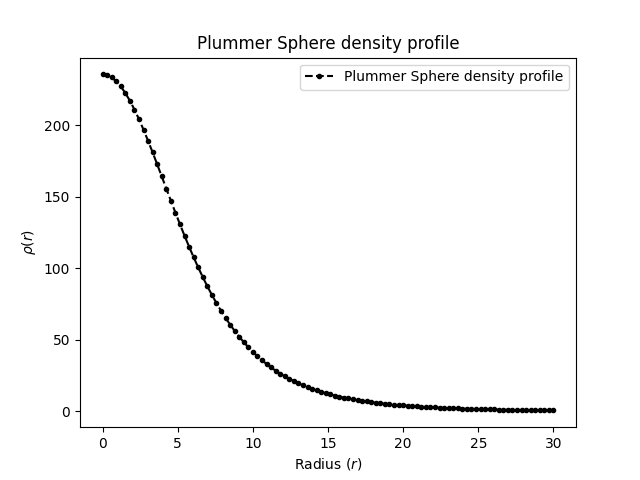
\includegraphics[width = 0.85\textwidth]{images/Plummer Sphere density profile.png}
\caption{Plummer sphere density profile}
\end{minipage}

\heading{Generation of mock catalogue}
\begin{itemize}
    \item Generate particles in the \textit{spatial subspace} as a random realisation of the plummer sphere mass distribution.
    \item Assign each particle a velocity vector in the \textit{velocity subspace} such that the velocity distribution follows the energy distribution function.
\end{itemize}
\subheading{\textbf{Populating \textit{spatial subspace}}} \\
Cumulative mass distribution function for plummer sphere is given by 
\begin{equation}\label{eq:plummer_mass_distribution}
    M(r) = \displaystyle{\int_0^{\infty} 4\pi r^2 \rho(r) dr  }  = \displaystyle{\frac{M_0r^3}{(r^2 + b^2)^{3/2}}} = \displaystyle{\frac{M_0 (r/b)^3}{(1 + r^2/b^2)^{3/2}}}
\end{equation}
Using the above relation, one can solve for $r(m)$ as
\begin{equation}\label{eq:plummer_inverse_mass_distribution}
\boxed{r(m) = \displaystyle{\frac{b}{\sqrt{(M_0/m)^{-2/3}-1}}}}
\end{equation}
Particles can be arranged as a random realisation of eqn.\ref{eq:plummer_inverse_mass_distribution} \\ \\ 
. \\
. \\

\subheading{\textbf{Spatial subspace plot of plummer sphere mock catalogue}}


\begin{columns}[T] % align columns
\begin{column}{.48\textwidth}
\color{black}\rule{\linewidth}{4pt}
Density Profile plot
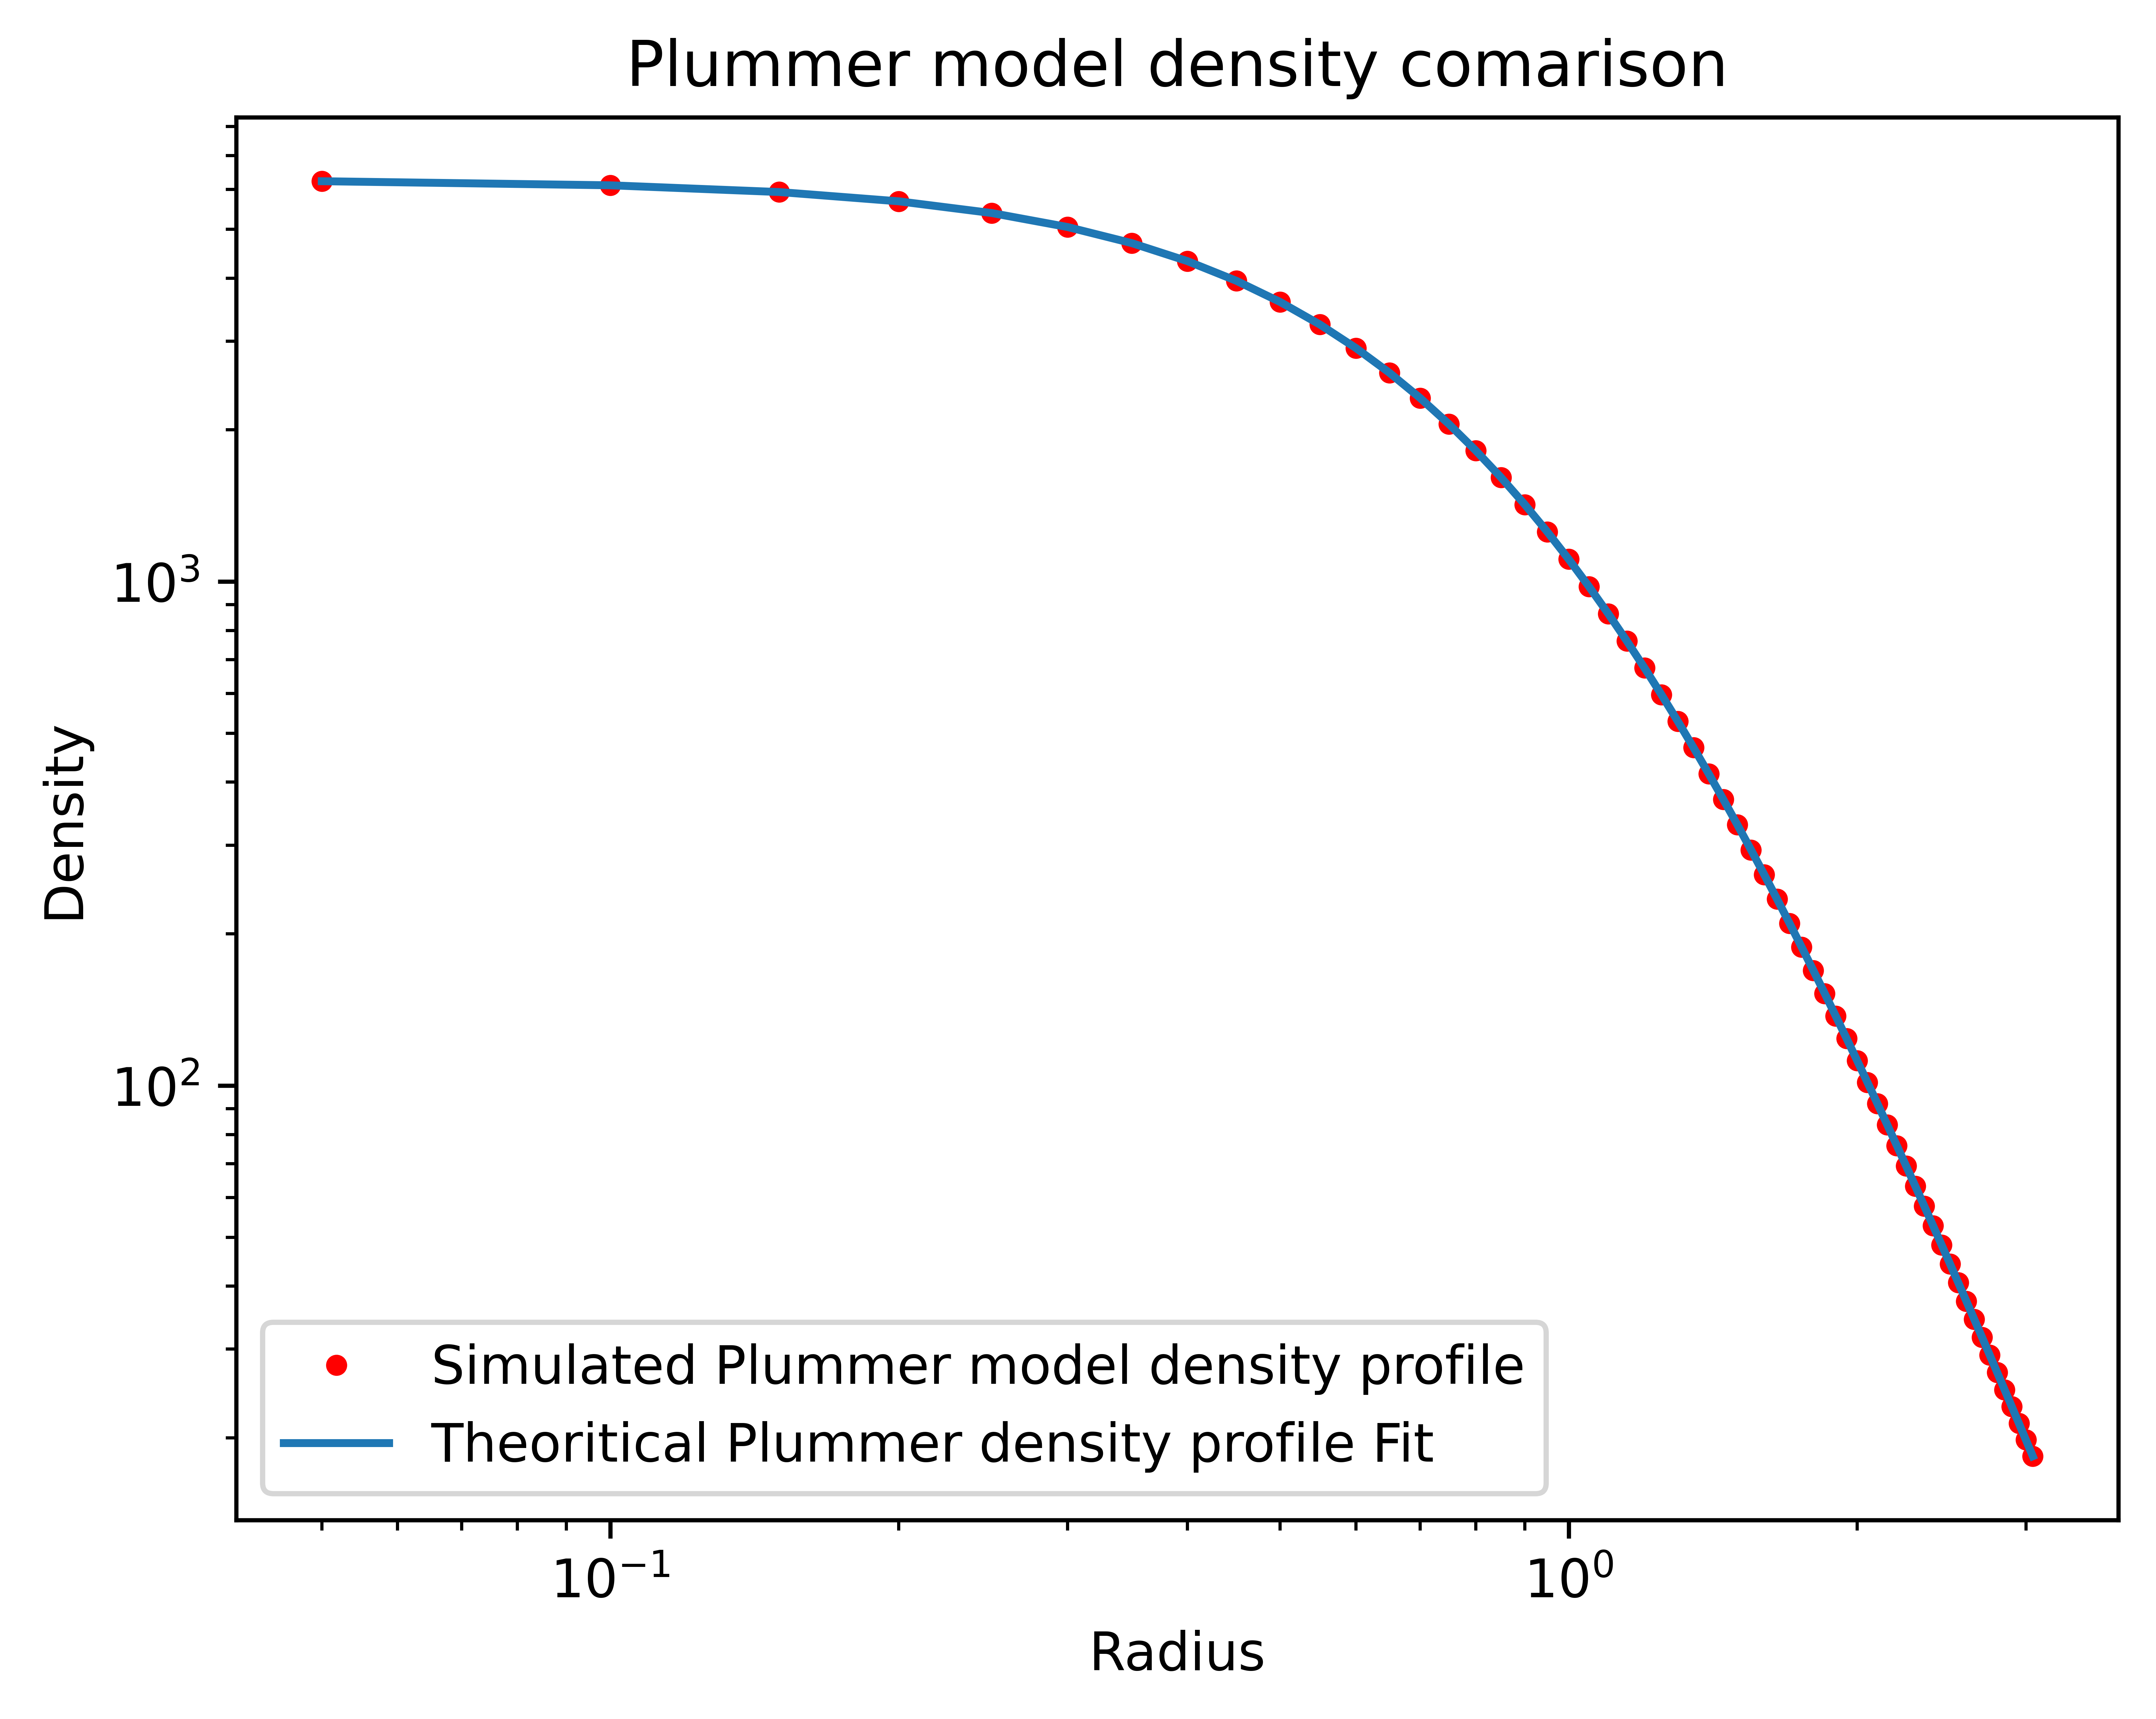
\includegraphics[width = 0.65\textwidth]{log_density.png}
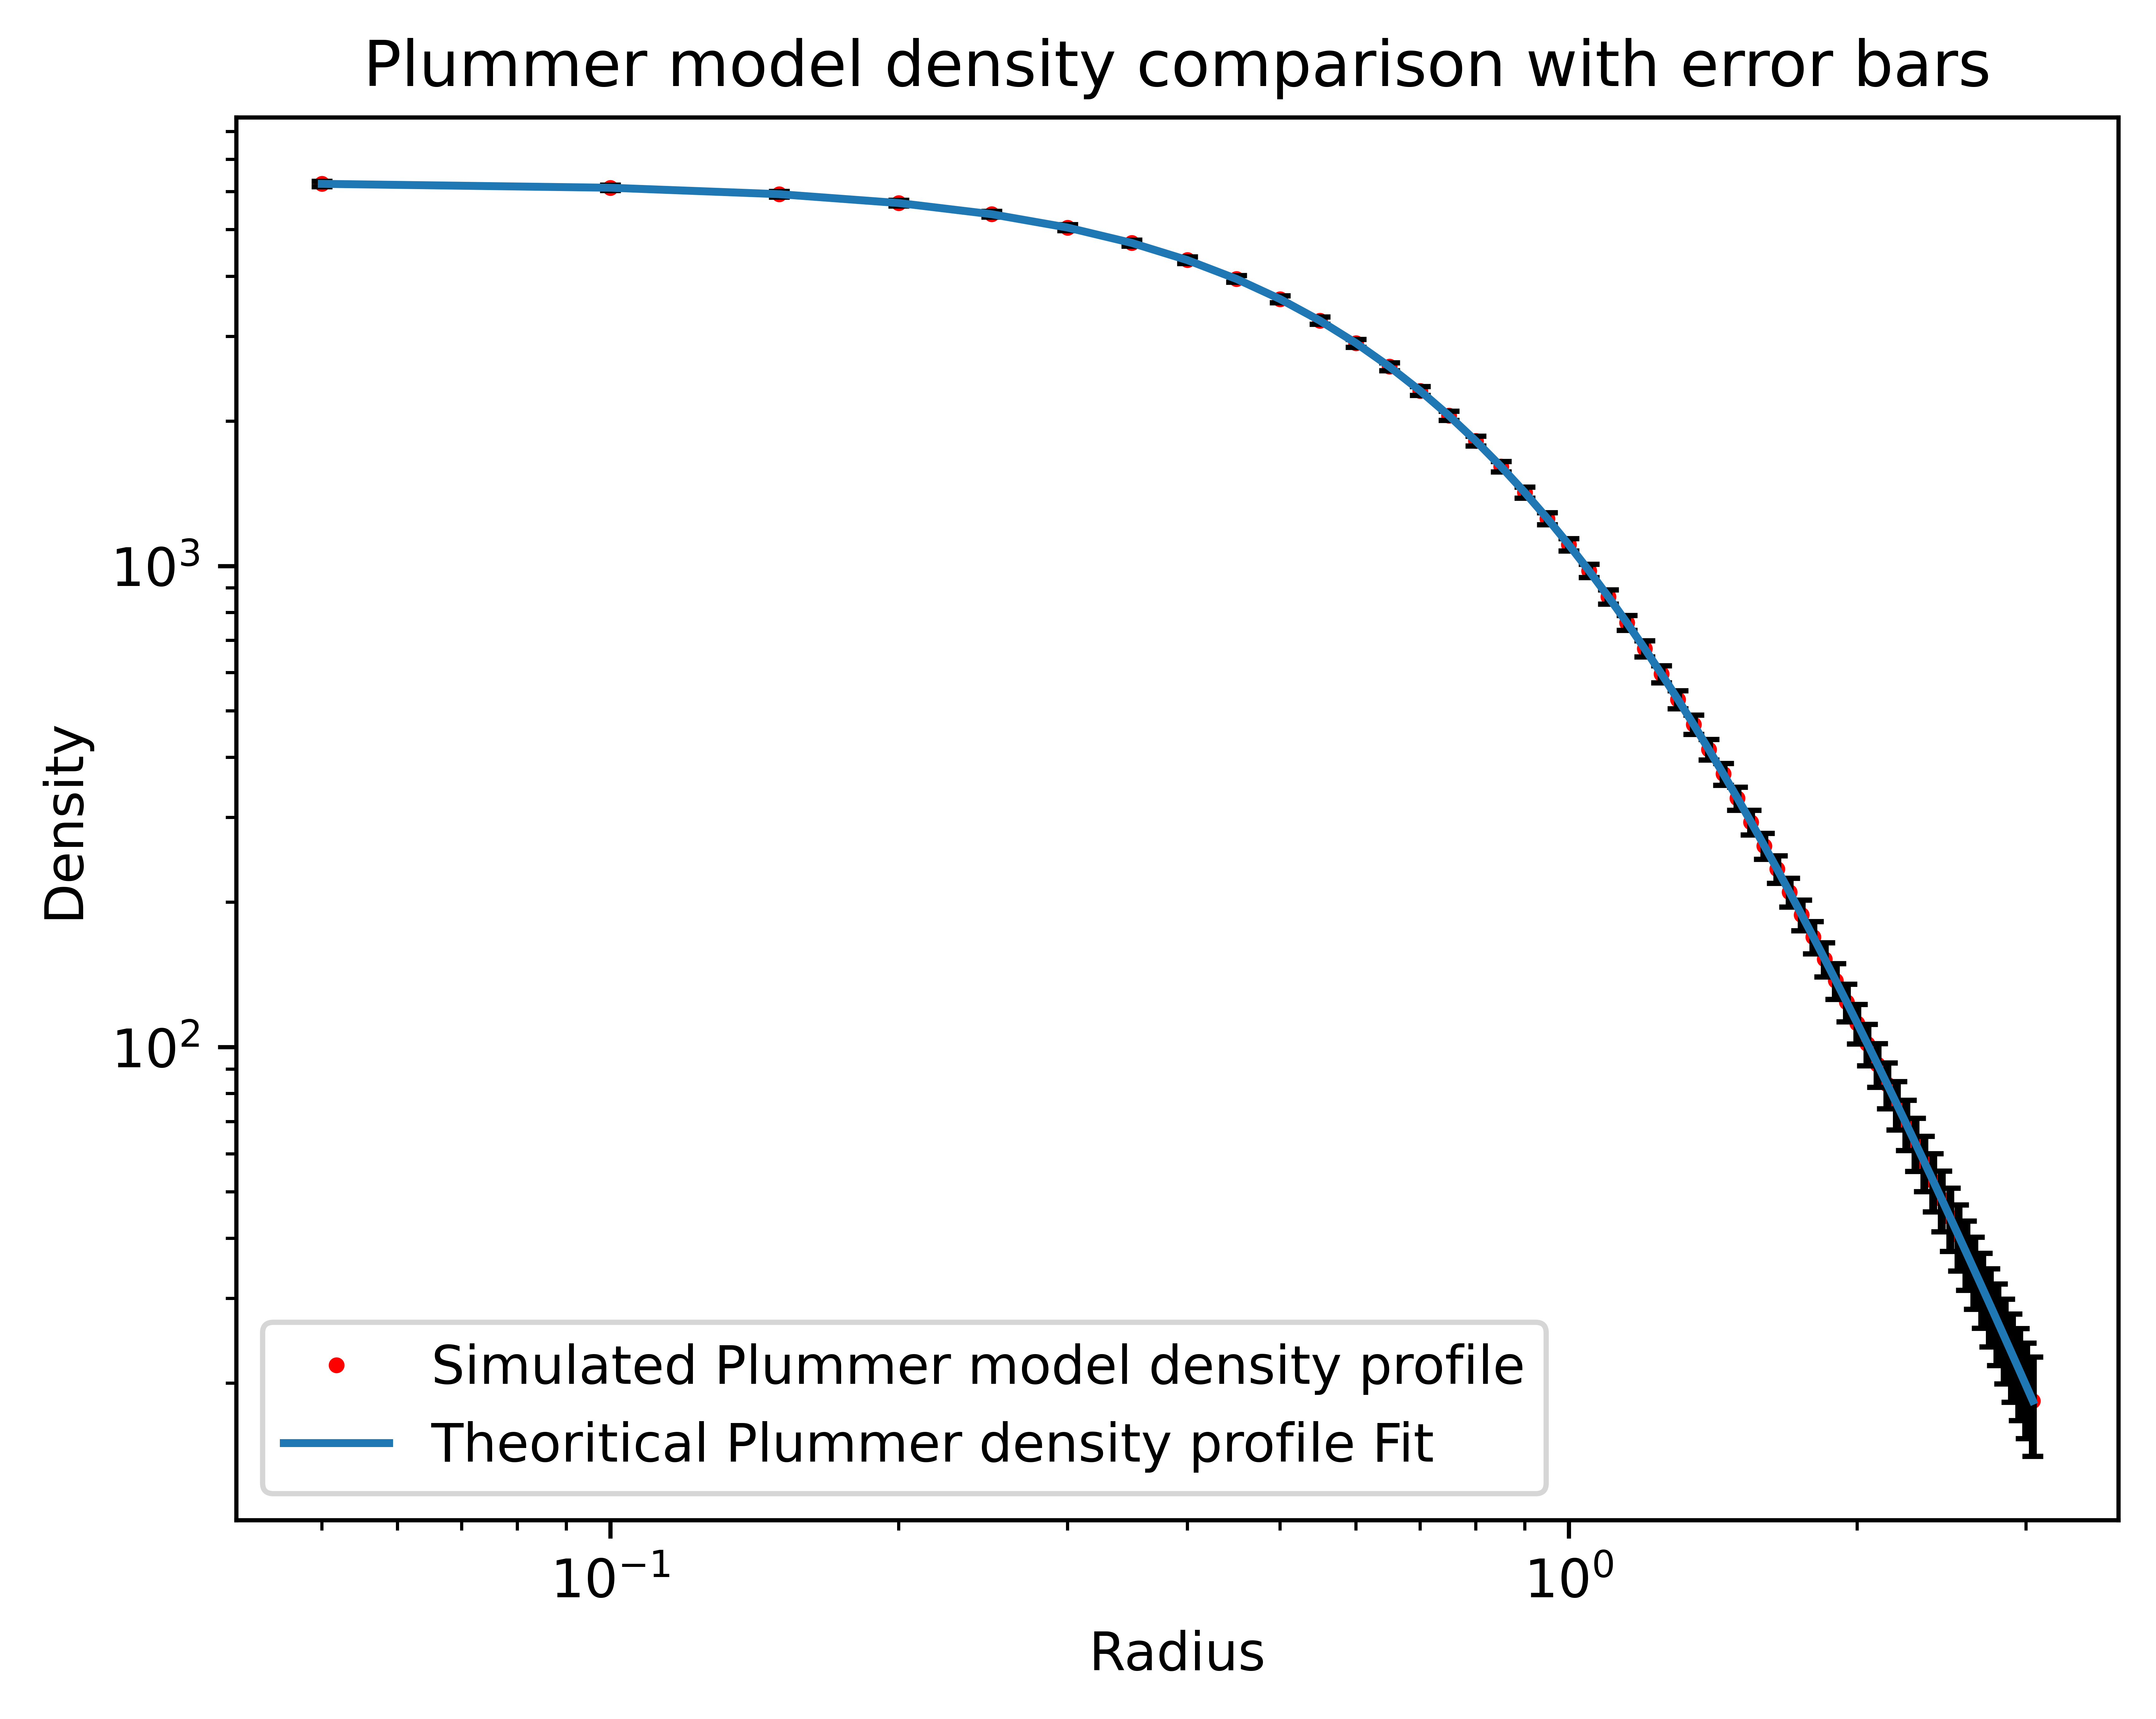
\includegraphics[width = 0.65\textwidth]{log_density_error.png}


\end{column}%
\hfill%
\begin{column}{.48\textwidth}
\color{black}\rule{\linewidth}{4pt}

Plummer Sphere 2D Projection 
. \\
. \\
. \\
. \\
. \\

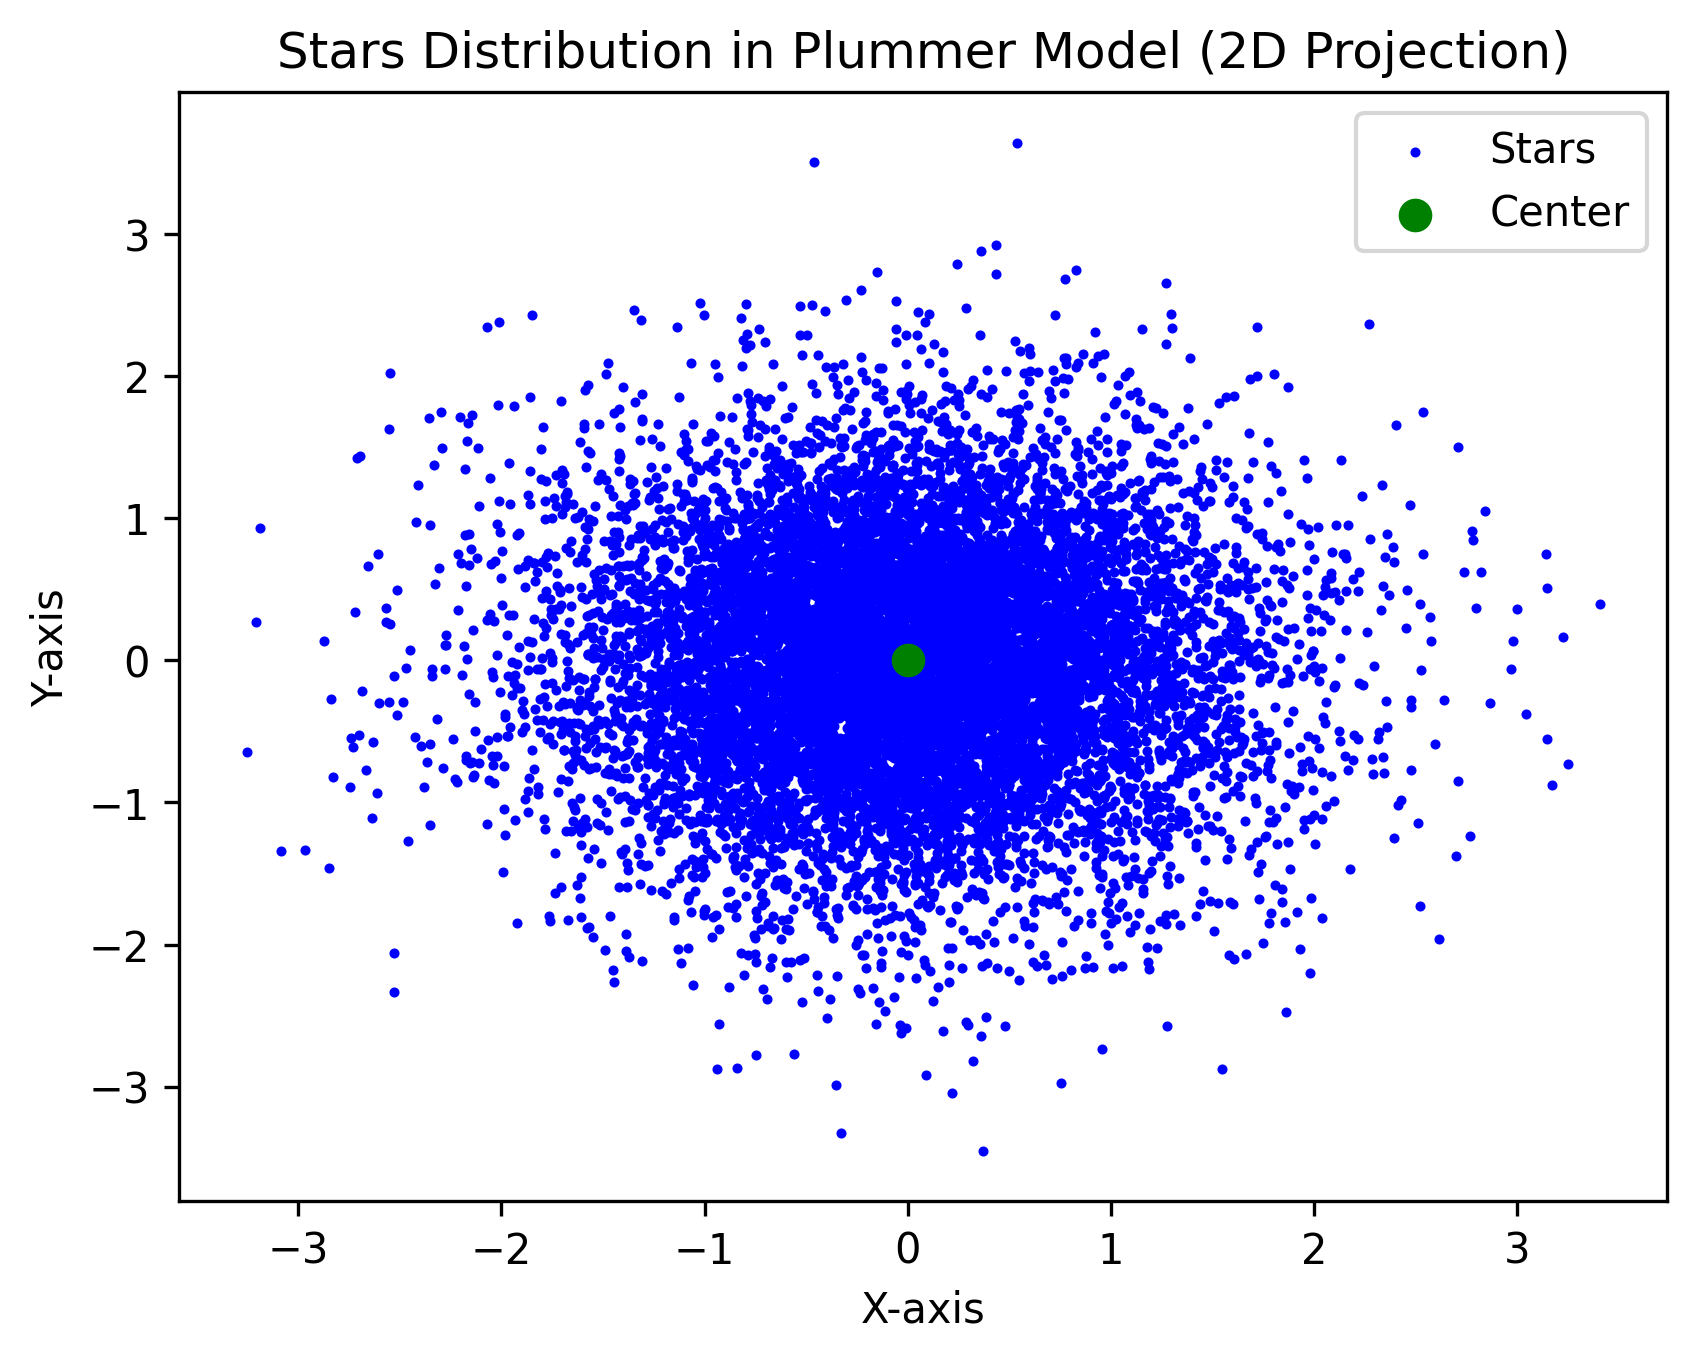
\includegraphics[width = 0.85\textwidth]{plummer_2d.png}
\end{column}%
\end{columns}


\subheading{\textbf{Populating \textit{velocity subspace}}} \\
Energy distribution function for particles in plummer sphere is 
\begin{equation}
    f(\Vec{r},\Vec{v})d\Vec{r}d\Vec{v} = f(E(r,v))4\pi r^2 dr 4\pi v^2 dv = \displaystyle{\frac{384\sqrt{2}}{7\pi m}} (-E)^{7/2} r^2 v^2 dr dv  
\end{equation}
Transforming the above equation for the magnitude of velocity , we get 
\begin{equation}\label{eq:vel_pdf}
    g(q) = (1 - q^2)^{7/2}q^2 \text{ where } q = \displaystyle{\frac{v}{v_e}}
\end{equation}
Looks similar to random realisation problem, but analytical inverse of eqn.\ref{eq:vel_pdf} doesn't exists. Using \textit{Jon Von Neumann rejection technique} one can solve for $q$ and hence for $v(r)$ as 
\begin{equation}
    \boxed{v = q \times v_e \implies v(r) = \sqrt{2} q (r^2 + 1)^{-1/4}}
\end{equation}

  \end{block}

% ----------------------------------
% Section: Study methodology
% ----------------------------------
%  \begin{block}{Study methodology}
%     % The present study adopted the following step-by-step methodology to achieve the research objectives.
 
%     % % This flow chart is created by the author

% adjustbox is used to limit the figure inside the page
% -- means normal arrow
%  -| horizontal followed by the vertical arrow
%  |- vertical followed by the horizontal arrow


\begin{figure}

    \begin{center}
        \begin{adjustbox}{max height=0.7\textheight, center, width=0.8\textwidth}
            \begin{tikzpicture}[node distance=3cm]
                \node (step1_1) [startstop] {\textbf{Innulla risus}};
                \node (step1_2) [process, below of = step1_1] {\textbf{Lorem ipsum}};
                \node (step1_3) [process, below of = step1_2] {\textbf{Suspendisse potenti}};
                \node (step1_4) [process, below of = step1_3] {\textbf{Morbi odio velit}};

% ---------------------------------------------
% vertical (primary) Division
% ---------------------------------------------
                % Flow

                \node (step1_5) [process, below of = step1_4, yshift = -1cm] {\textbf{Suspendisse a}};

                \node (step1_6) [process, below of = step1_5, yshift = -0.7cm] {\textbf{Maecenas velit lectus}};

                \node (step1_7) [process, below of = step1_6, yshift = -1.3cm] {\textbf{Suspendisse a}};

                \node (step1_8) [process, below of = step1_7, yshift = -0.7cm] {\textbf{Pellentesque pulvinar}};

                \node (step1_9) [process, below of = step1_8, yshift = -0.2cm] {\textbf{Nam ullamcorper}};

                \node (step1_10) [process, below of = step1_9, yshift = -0.2cm] {\textbf{Phasellus}};


% ---------------------------------------------
% All arrows (for vertical column
% ---------------------------------------------

                %  All arrows (for vertical column
                \draw [arrow] (step1_1) -- (step1_2);
                \draw [arrow] (step1_2) -- (step1_3);
                \draw [arrow] (step1_3) -- (step1_4);
                \draw [arrow] (step1_4) -- (step1_5);
                \draw [arrow] (step1_5) -- (step1_6);
                \draw [arrow] (step1_6) -- (step1_7);
                \draw [arrow] (step1_7) -- (step1_8);
                \draw [arrow] (step1_8) -- (step1_9);
                \draw [arrow] (step1_9) -- (step1_10);

% ---------------------------------------------
% Left Division
% --------------------------------------------- 
                \node (step2_1) [process, left of = step1_4, xshift=-10cm, yshift=-2.6cm] {\textbf{Cras sem felis Cras sem felis}};

                \node (step2_2) [process, below of = step2_1, yshift=-0.8cm] {\textbf{Pellentesque pulvinar}};

                \node (step2_3) [process, below of = step2_2, yshift=-0.4cm] {\textbf{Suspendisse potenti}};
                

% ---------------------------------------------
% All arrows (for the left column)
% ---------------------------------------------

                %  All arrows (for vertical column
                \draw [arrow] (step1_4) -| (step2_1);
                \draw [arrow] (step2_1) -- (step2_2);
                \draw [arrow] (step2_2) -- (step2_3);
                \draw [arrow] (step2_3) |- (step1_7);

% ---------------------------------------------
% Right Division
% ---------------------------------------------   
                \node (step3_1) [process, right of = step1_7, xshift=10cm, yshift=-5cm] {\textbf{Suspendisse potenti}};

% ---------------------------------------------
% All arrows (for right column)
% ---------------------------------------------

                %  All arrows (for vertical column
                \draw [arrow] (step1_7) -| (step3_1);
                \draw [arrow] (step3_1) |- (step1_10);
                
            \end{tikzpicture}
        \end{adjustbox}
    \end{center}
    \caption{Caption for flowchart.}
    \label{fig:figure1}
\end{figure}

%  \end{block}

% % -------------------------------
% % Section: Site selection and data collection
% % -------------------------------
% \begin{block}{Site selection and data collection}
 
    
% \end{block}

% % -------------------------------
% % Section: Descriptive Statistics
% % -------------------------------

% \begin{block}{Descriptive statistics}
%     \begin{itemize}
%         \item Sed et augue accumsan nibh 45\% ullamcorper accumsan.
%         \item Sed et augue accumsan nibh ullamcorper accumsan. Nam dictum urna tortor, ut pretium leo eleifend efficitur. 
%         \item Nullam at velit facilisis nibh vulputate porta a sit amet metus.
%         \item Maecenas eget nunc suscipit, luctus nisl non, tristique felis.
%         \item Maecenas tellus diam, placerat sit amet nisl at, dapibus imperdiet arcu.
%     \end{itemize} 
% \end{block}


  \begin{block}{References}

    \nocite{*}
    \footnotesize{\bibliographystyle{plain}\bibliography{poster}}

  \end{block}


\end{column}

\separatorcolumn

\begin{column}{\colwidth}

% -------------------------------
% Section: Results and discussion
% -------------------------------

\begin{block}{NBody simulations}
We conducted N-Body simulations on our numerically generated Plummer sphere, as well as upon introducing a black hole within the Plummer sphere, in order to comprehensively examine the underlying dynamics of these systems. We used \textit{Barnes-Hut algorithm} for NBody simulations.
    \heading{Barnes-Hut algorithm}
The Barnes-Hut algorithm is a hierarchical, tree-based method for approximating N-body simulations, which significantly reduces computational complexity. By dividing the simulation space into a hierarchical structure called an octree (in 3D) or quadtree (in 2D), it enables the calculation of gravitational interactions among particles with a time complexity of $\mathcal{O}{N \log N}$ instead of the standard $\mathcal{O}{N^2}$ required for direct methods. A very brief summary of how this algorithm works is listed below:
\begin{enumerate}
    

 \item  \textbf{Initialisation of populating the octree structure} \\
 \begin{itemize}
        \item Vertical cubical division of empty space into sub(cells)
        \item Construction of the tree structure by 
        \begin{itemize}
            \item Discarding empty subcells 
            \item Accepting subcells with only one occupant
            \item Recursively dividing subcells with shared occupancy
        \end{itemize}
        \item Performing this tree construction \textit{"ab-initio"} every time.
    \end{itemize}

\item \textbf{Force calculation} \\
The interaction between the particle and the cluster of particles is determined by the hyper-parameter called $\theta$ defined as ratio of length of cell to the distance between particle and cluster. The force terms are calculated by taylor expanding cluster potential around its center of mass and is given by the following eqn. 
\begin{equation}\label{eq:quadrupole_potential_acceleration}\boxed{
                  \vec{a} = -GM \displaystyle{\frac{\hat{r}}{r^2} + \frac{G}{r^4}\vec{Q}\cdot\hat{r} - \frac{5G}{2}\left(\hat{r}\cdot \hat{r} \right) \frac{\hat{r}}{r^4}}}
\end{equation}
    \item \textbf{Update the position and velocity of each particle} \\
    One can employ various integrators, such as the Leapfrog integrator, to efficiently update the position and velocity of each particle following every time step, allowing for accurate and flexible simulation dynamics.
    
\end{enumerate}

\end{block}

% -------------------------------
% Section: Results
% -------------------------------
   \begin{block}{Results}
\heading{NBody simulation of plummer sphere}
We simulated the plummer sphere using \textit{Barnes-Hut algorithm} to establish the time-stationary nature of plummer sphere.  \\
\subheading{\textbf{Evolution and equilibrium of the system}} \\
% . \\

% 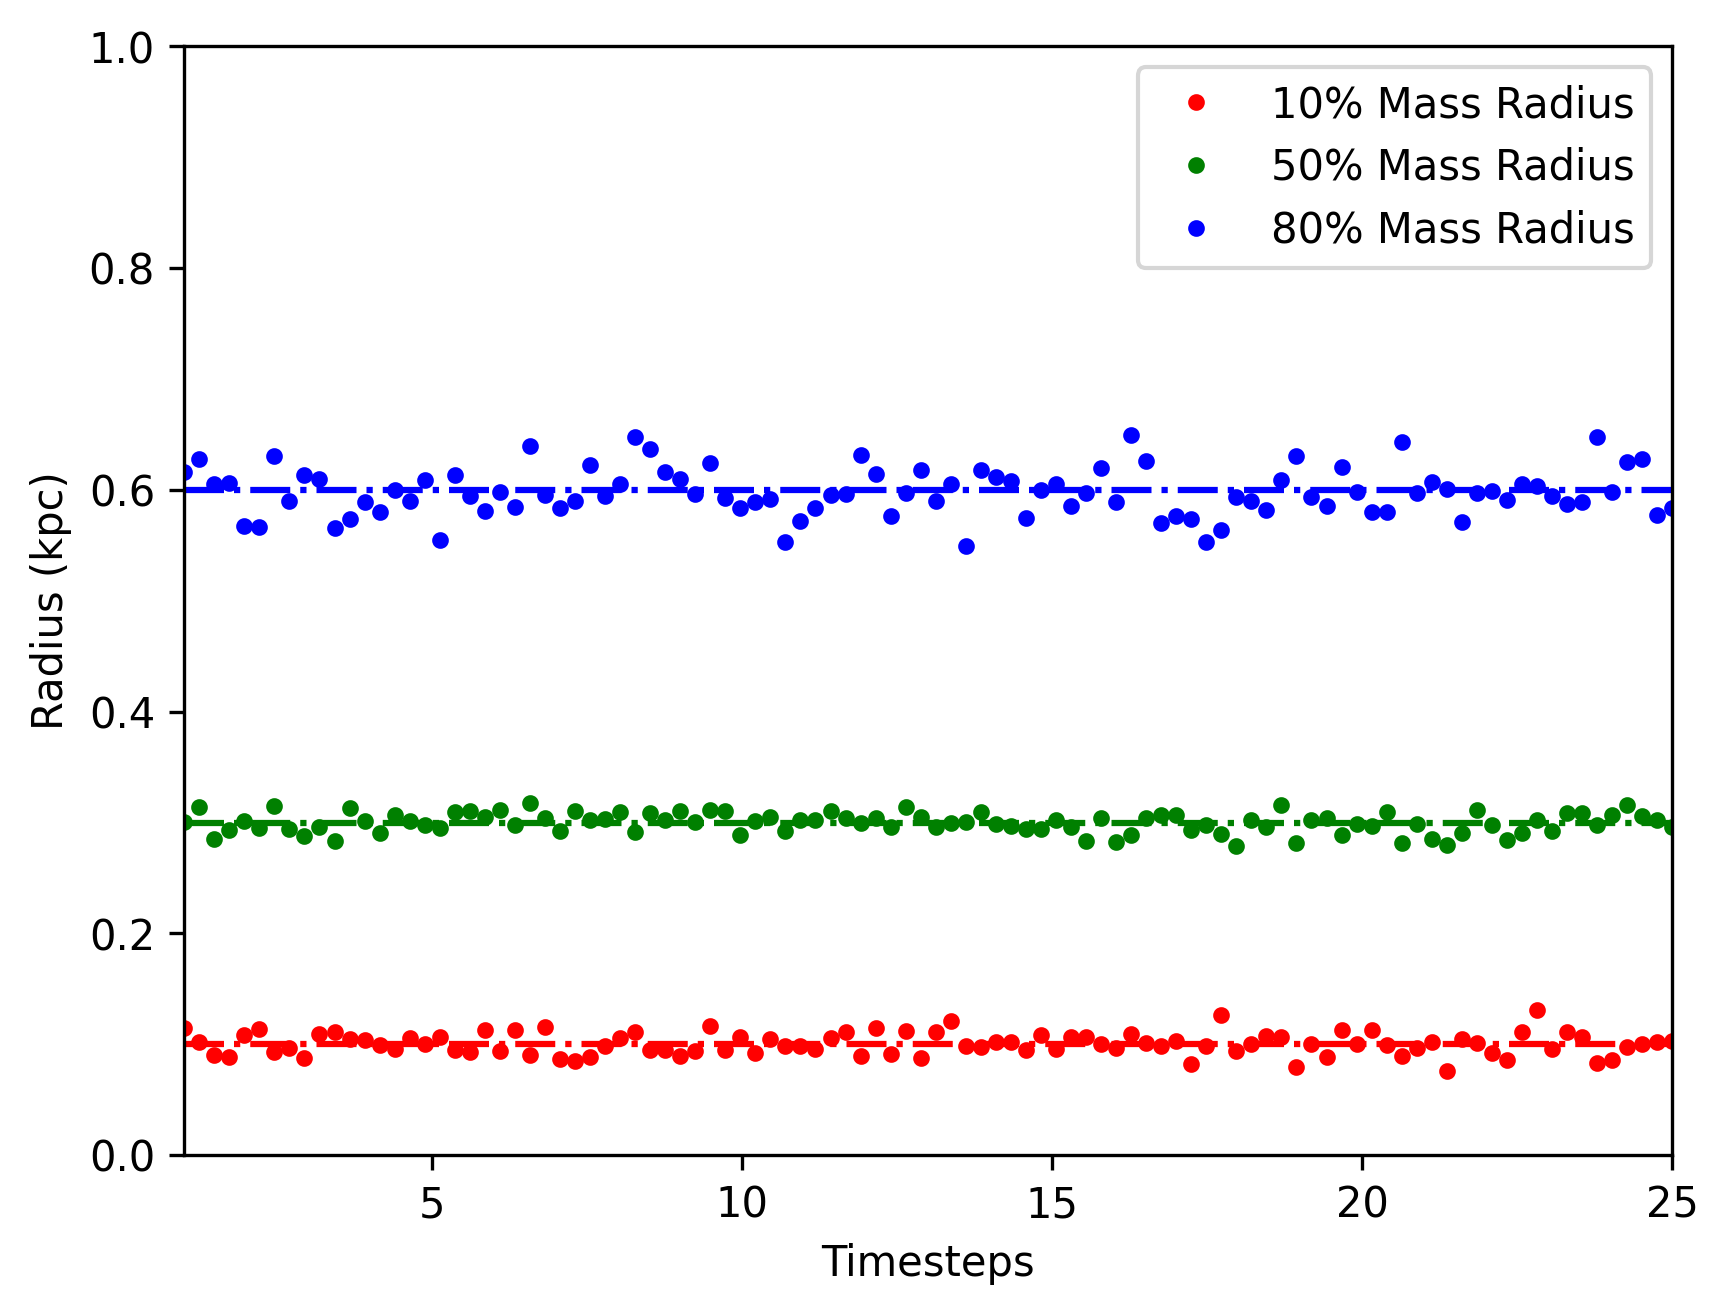
\includegraphics[width = 0.85\textwidth]{time-stationary.png}

\begin{columns}[T] % align columns
\begin{column}{.48\textwidth}
\color{blue}\rule{\linewidth}{4pt}
Snapshots
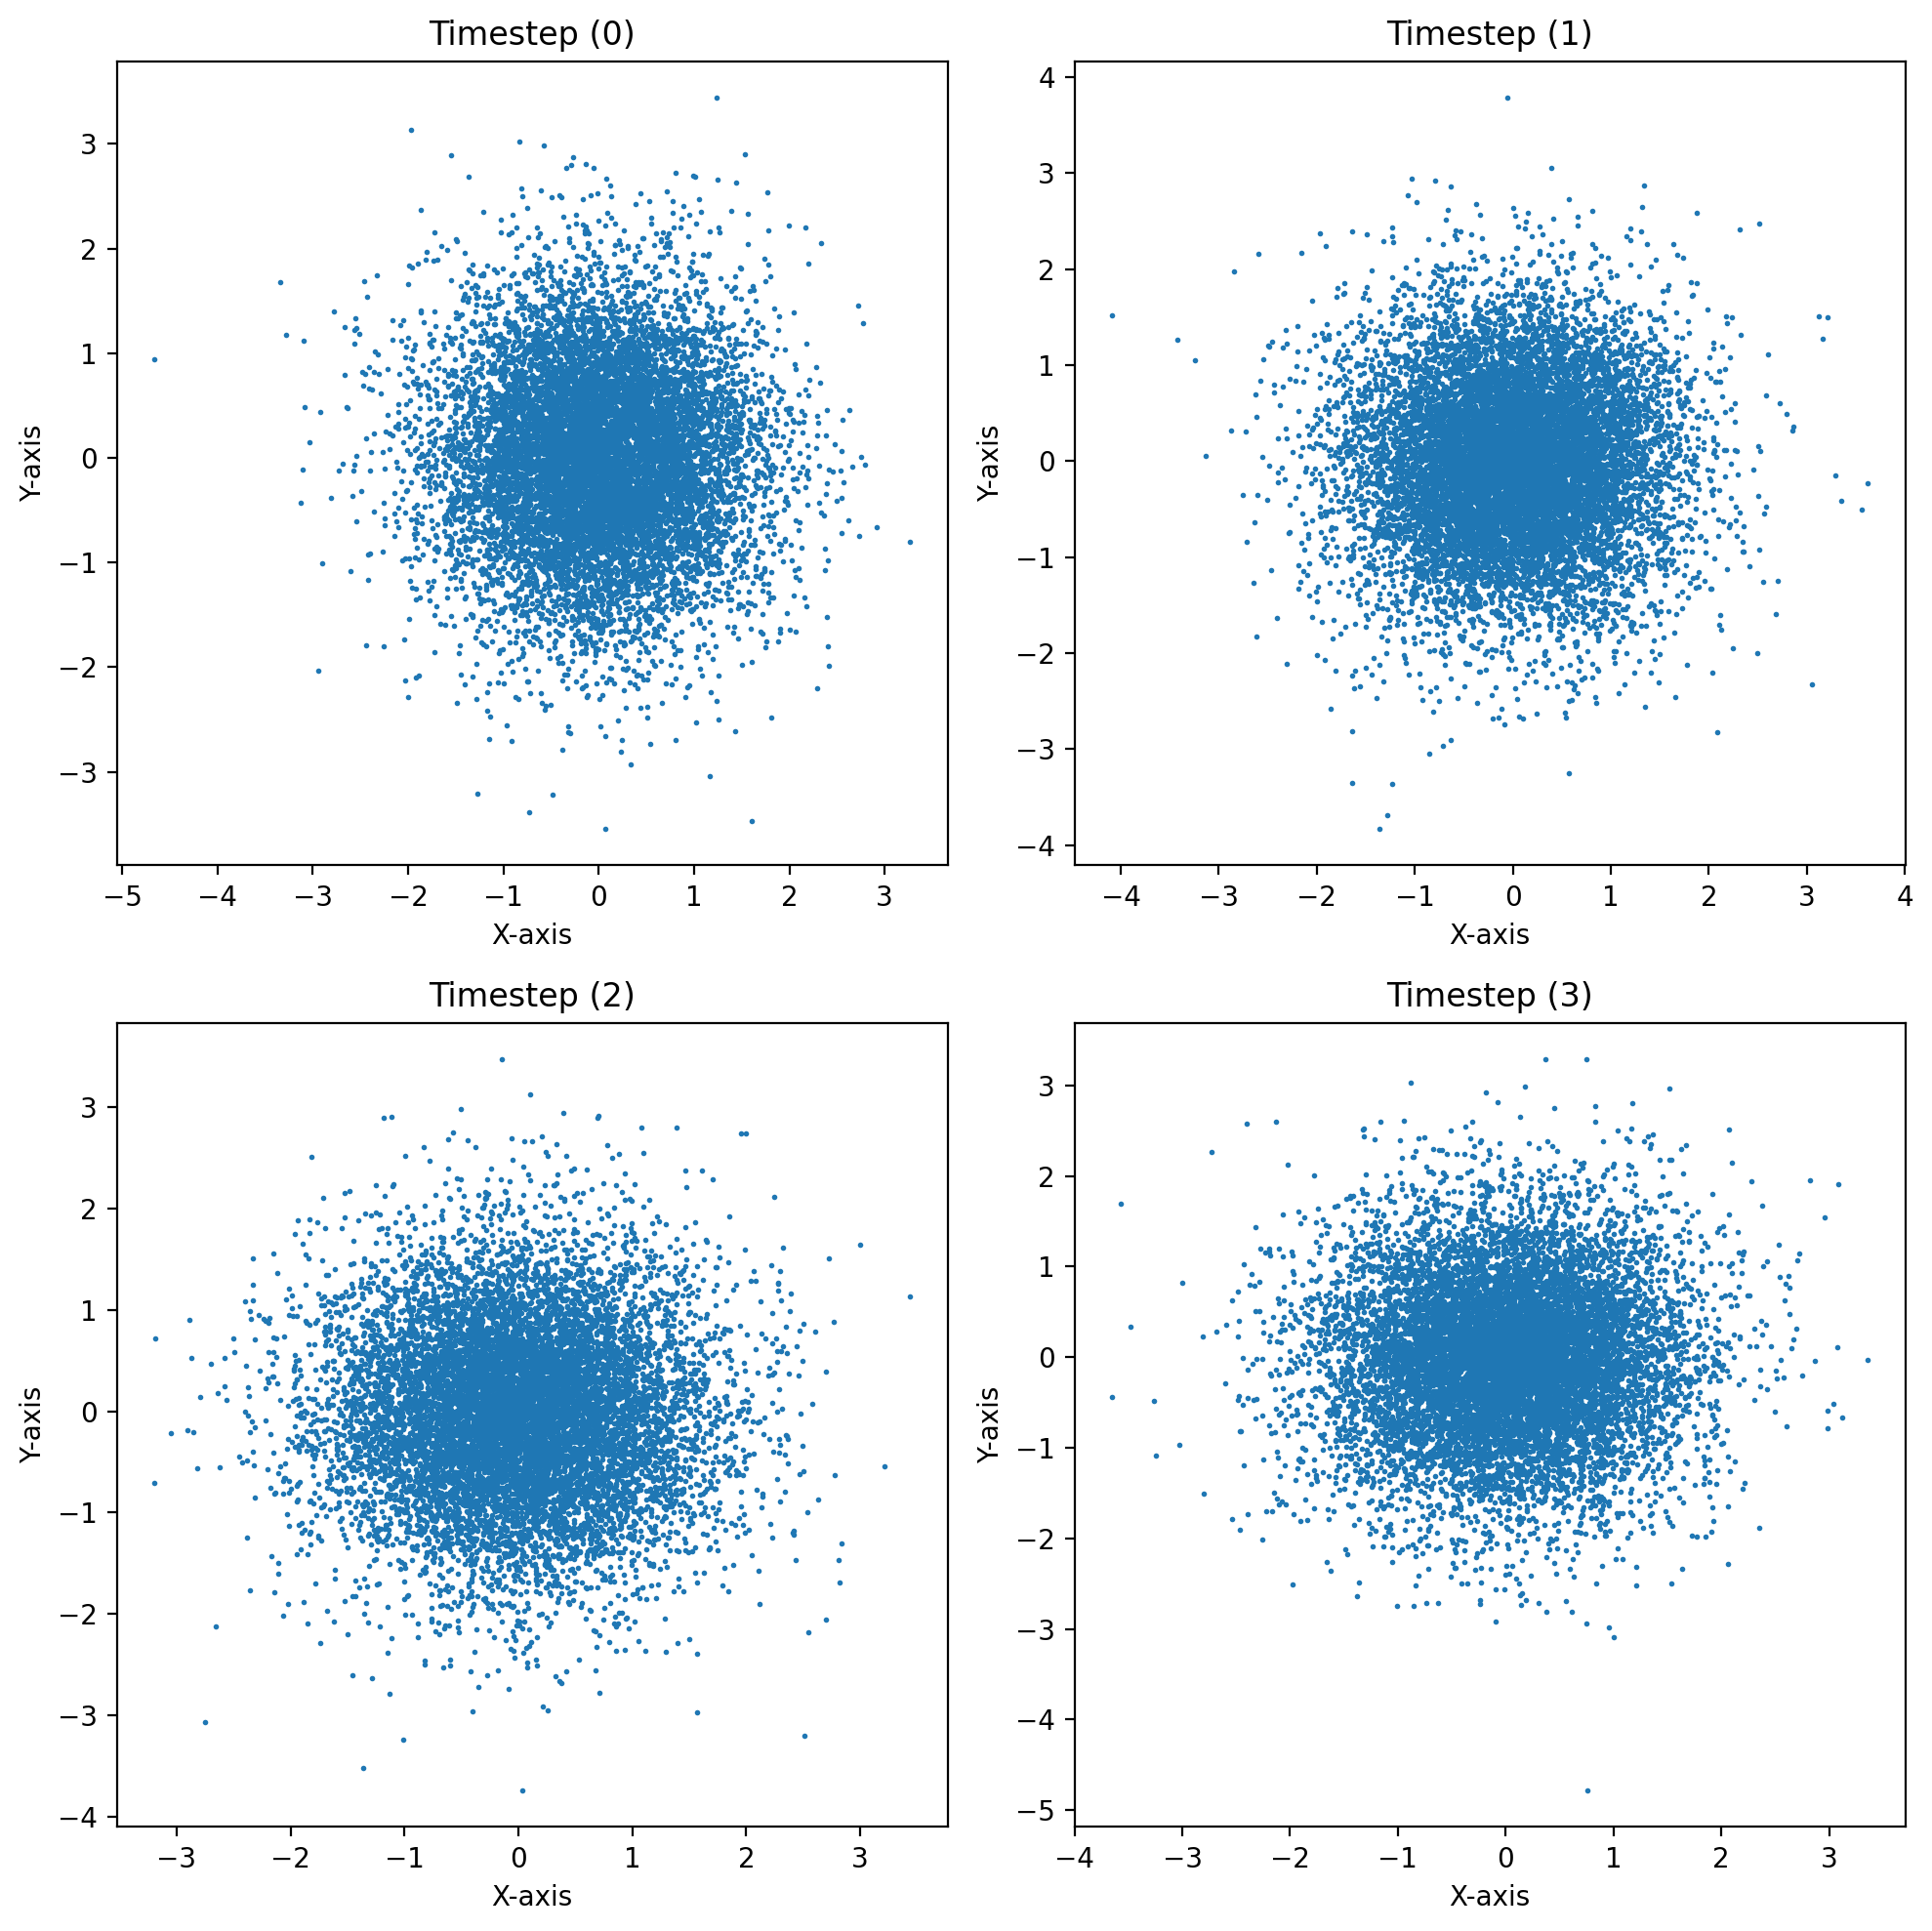
\includegraphics[width = 0.8\textwidth]{2d-stitched-plummer.png}
\caption{Simulation snapshots at different timesteps}
\end{column}%
\hfill%
\begin{column}{.48\textwidth}
\color{red}\rule{\linewidth}{4pt}
Plots
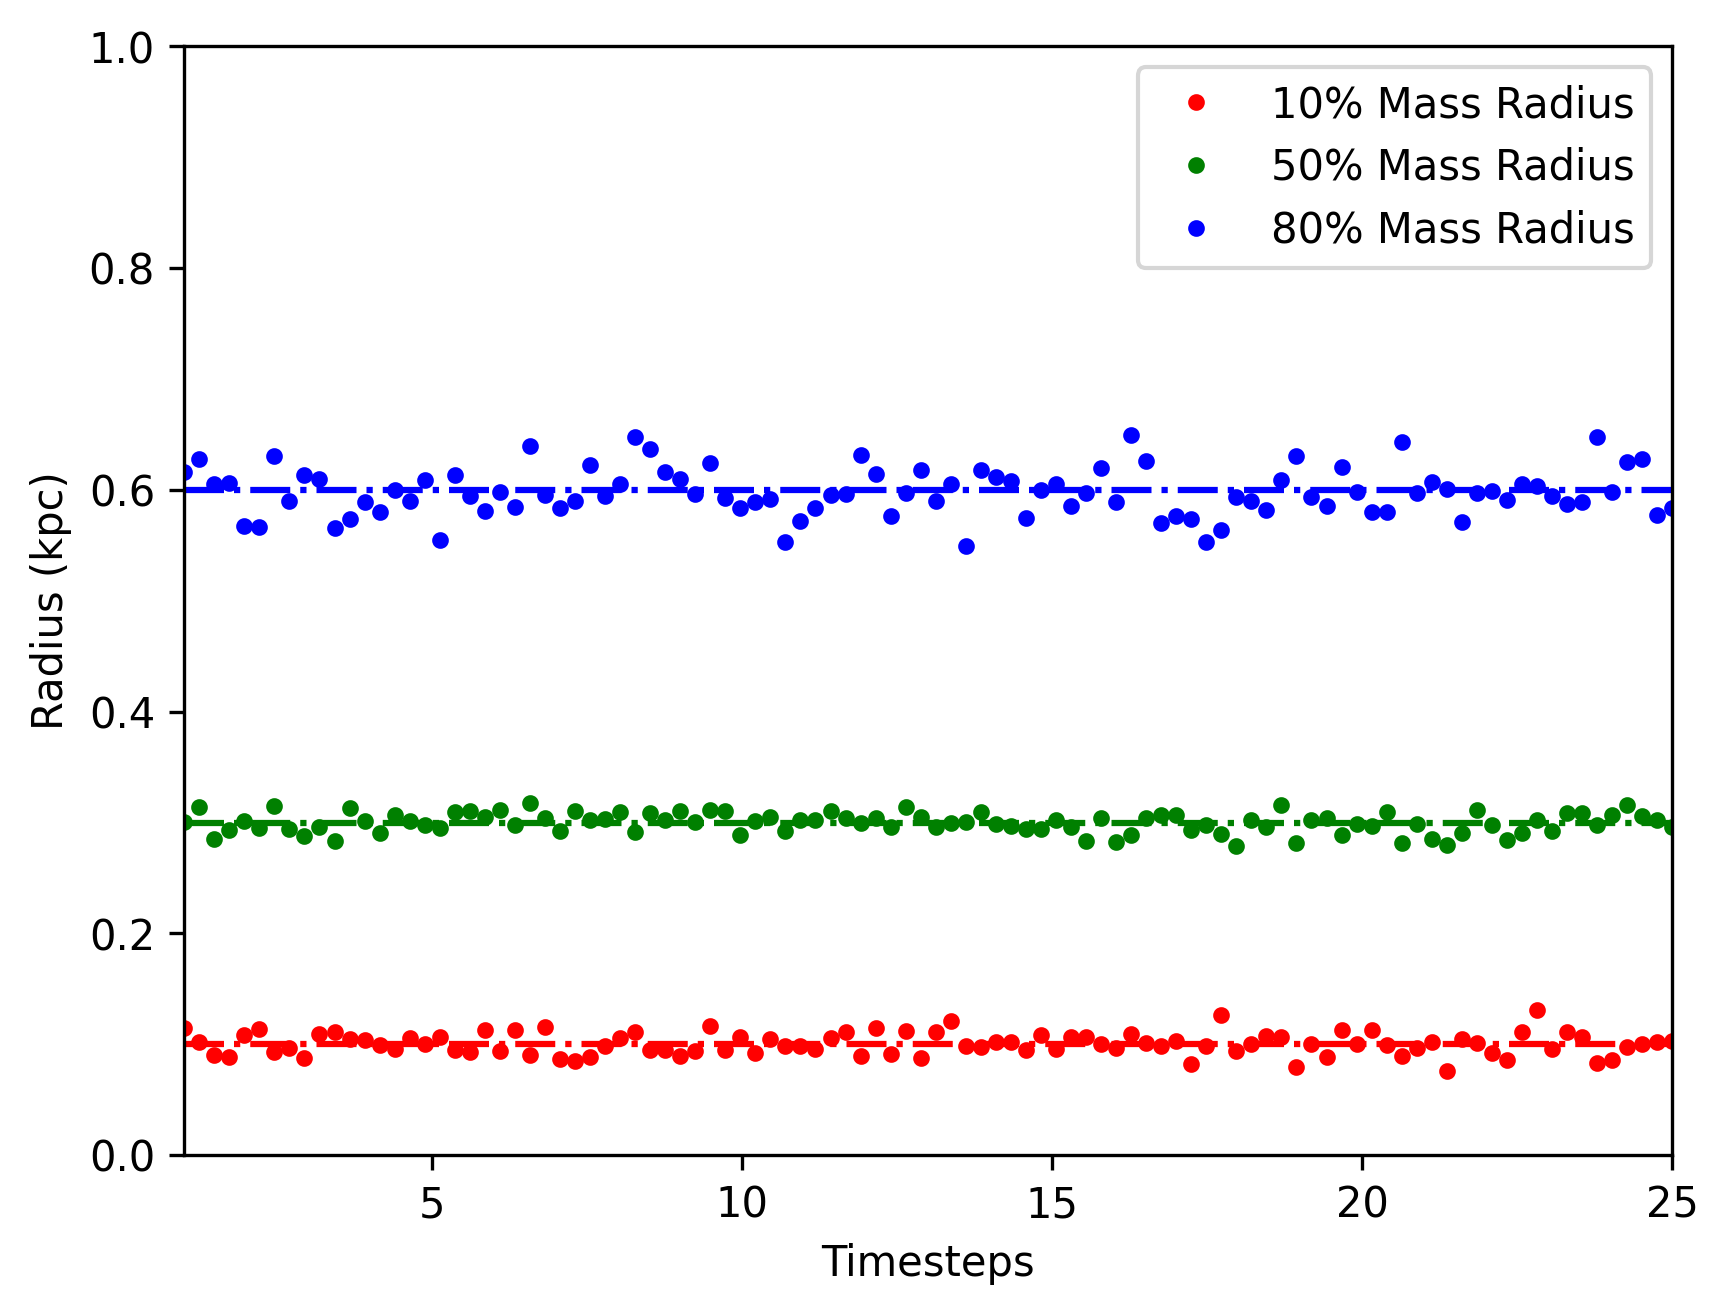
\includegraphics[width = 1.0\textwidth]{time-stationary.png}
\caption{Time stationary nature of the system}
\end{column}%
\end{columns}
 \\
 \heading{\textbf{NBody simulation of BH moving in plummer sphere}} \\
 We try to understand the dynamics of BH moving through the plummer by modeling its velocity profile under the influence of dynamical friction and compare it to the analytically calculated profile.
Analytical expression for a massive particle moving through a homogenous background of stars is given by 
\begin{equation}
    \boxed{\displaystyle{\frac{d \vec{v}_m}{dt}} = -16\pi^2 G^2 m_* (m + m_*) \log (\Lambda) \left[\int_0^{v_m} f(v_*)v^2_* dv \right] \displaystyle{\frac{\vec{v_m}}{v_m^3}} }
\end{equation}
  \end{block}
\\
\subheading{\textbf{Velocity profile of BH moving the cluster}}
\begin{columns}[T] % align columns
\begin{column}{.48\textwidth}
\color{blue}\rule{\linewidth}{4pt}
Analytical Velocity Profile
\begin{figure}
    \centering
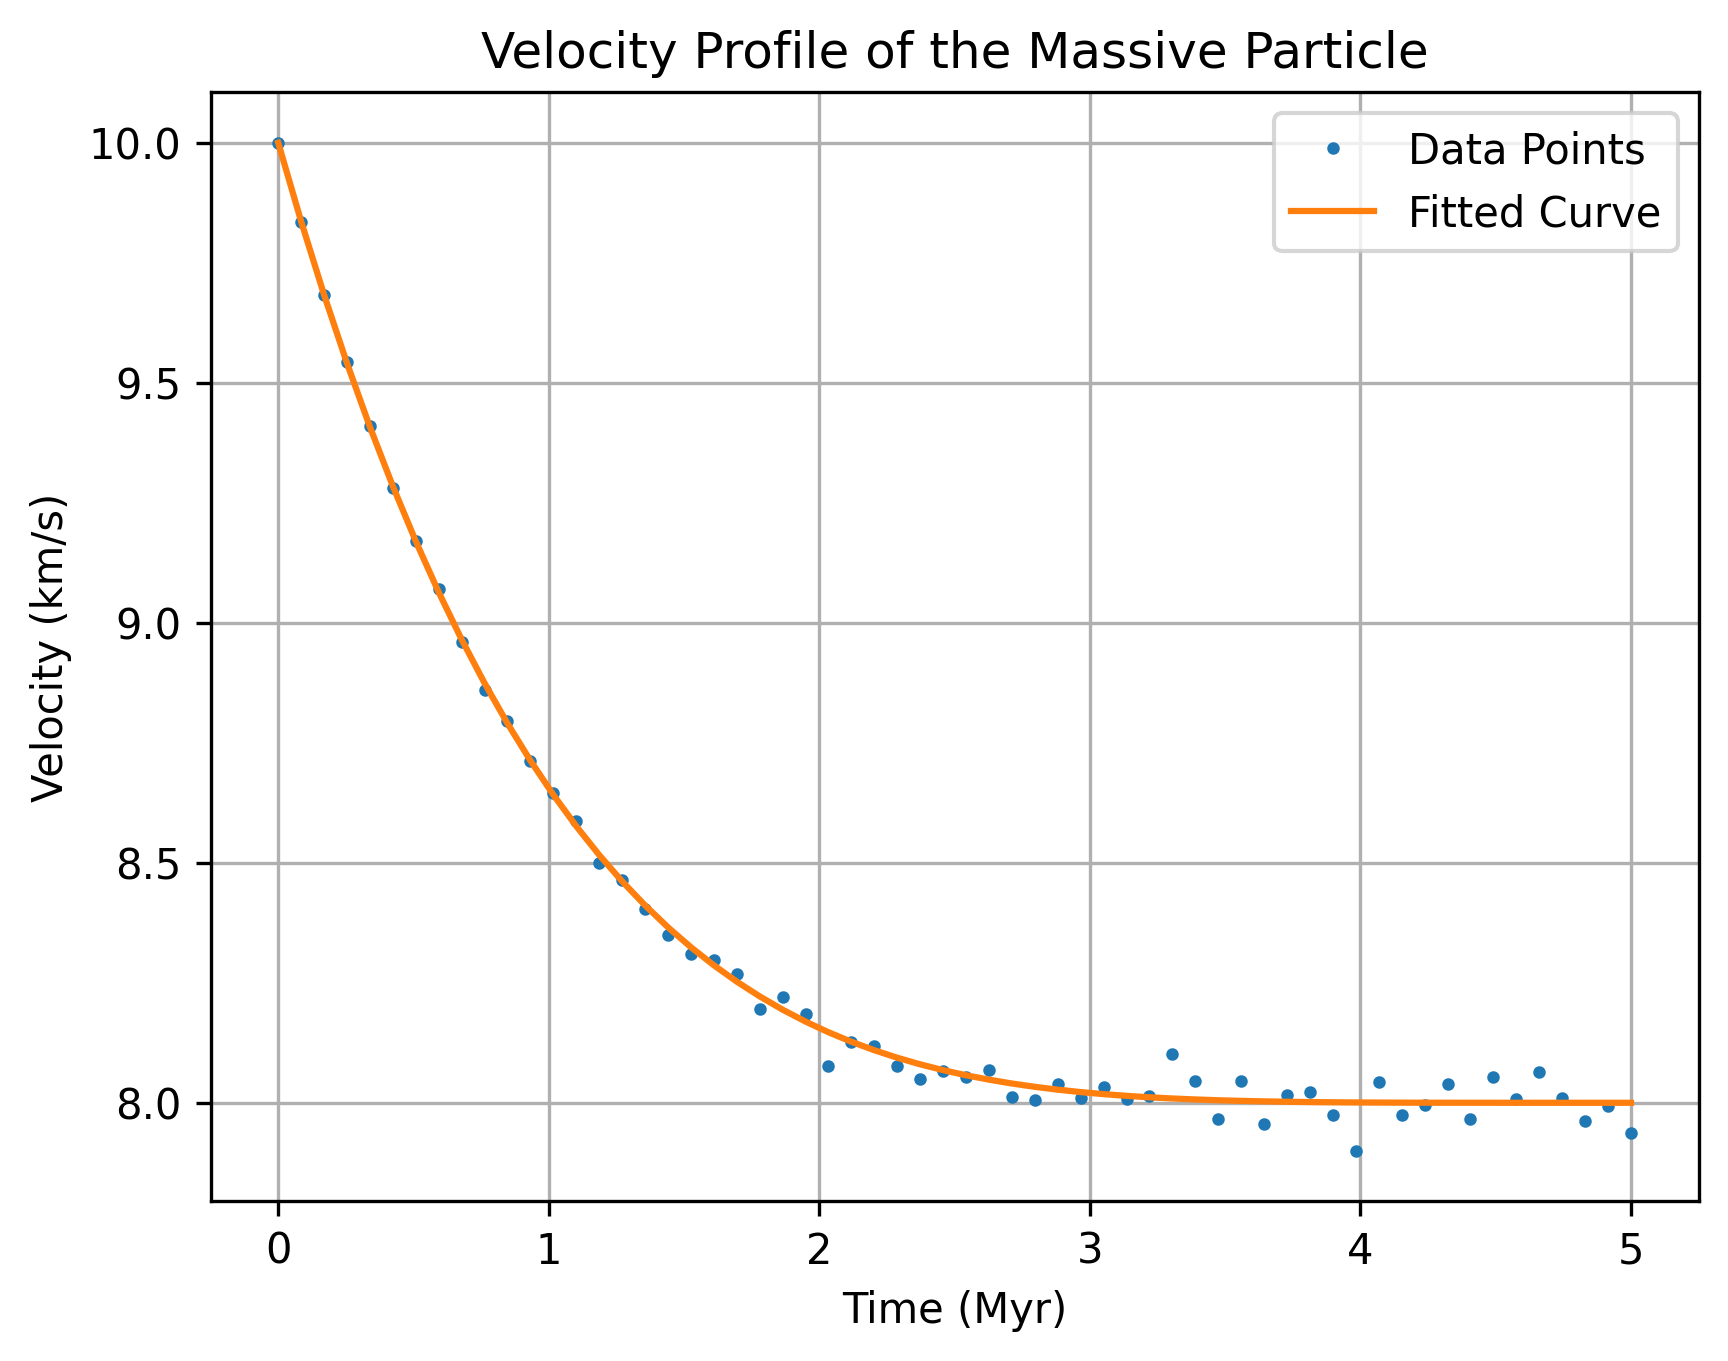
\includegraphics[width = 0.6\textwidth]{velocity_profile-vt-normal.png}
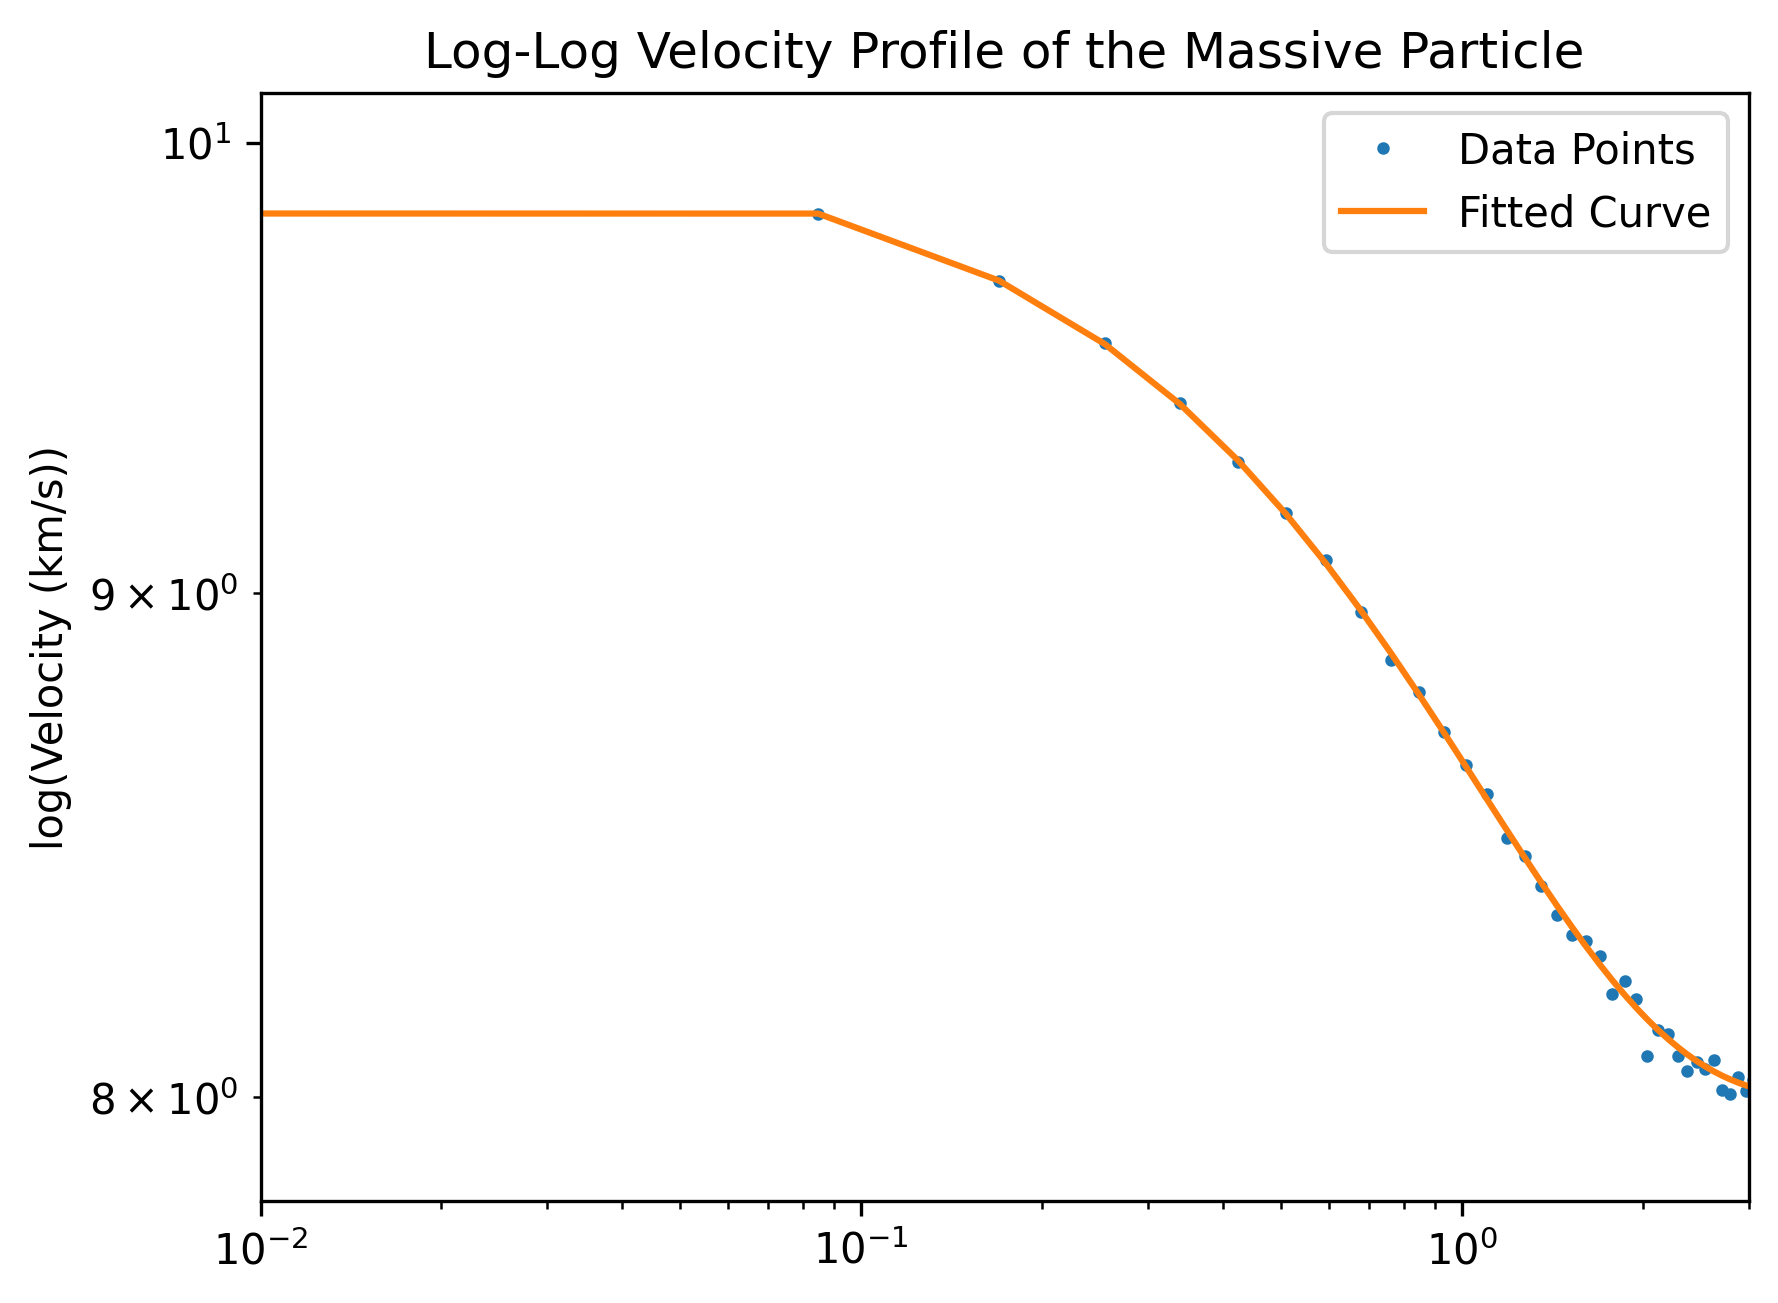
\includegraphics[width = 0.6\textwidth]{velocity_profile-vt-loglog.png}
\caption{Simulation snapshots at different timesteps}
    \label{fig:my_label}
\end{figure}

\end{column}%
\hfill%
\begin{column}{.48\textwidth}
\color{red}\rule{\linewidth}{4pt}
Numerical Velocity Profile
\begin{figure}
    \centering
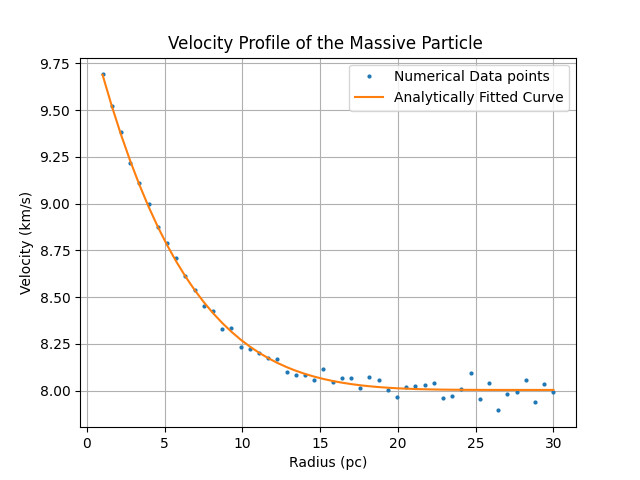
\includegraphics[width = 0.6\textwidth]{velocity-profile-vr-normal.png}
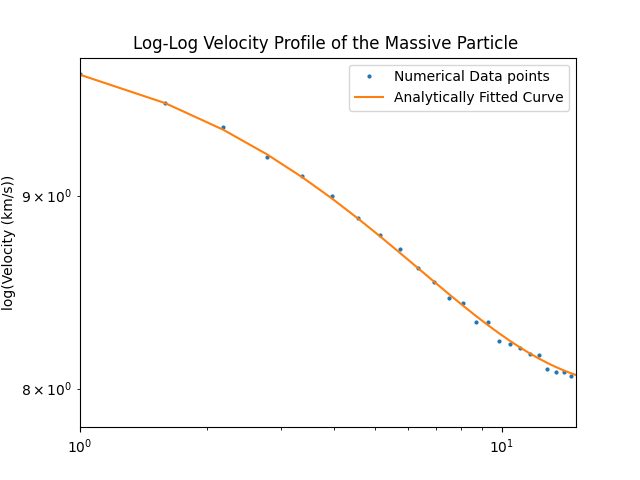
\includegraphics[width = 0.6\textwidth]{velocity-profile-vr-loglog.png}
\caption{Time stationary nature of the system}
    \label{fig:my_label}
\end{figure}

\end{column}%
\end{columns}



% -------------------------------
% Section: Practical Implications
% -------------------------------
  \begin{exampleblock}{Acknowledgement}
  I sincerely thank my supervisor Prof. Jasjeet Singh Bagla for his immense support and for his valuable suggestions throughout my thesis. I would also like to thank Dr Dipanweeta (PostDoc, TIFR Mumbai) for insightful suggestions which helped me a lot.

  \end{exampleblock}

% -------------------------------
% Section: References
% ------------------------------- 

% -------------------------------
% Section: Portfolio
% -------------------------------
  \begin{block}{Scan to view the digitised version}
    
    \begin{figure}[h]
    \centering
    
\includegraphics[width=0.1\textwidth]{images/portfolio.png}
    \caption*{Scan this QR code}
    \label{fig:figure3}
\end{figure}

  \end{block}

\end{column}
\separatorcolumn



\end{columns}
\end{frame}

\end{document}
